\chapter{Unsupervised learning: K-means and SOM}\label{ch-19}

This lecture is a light introduction to \textbf{unsupervised learning}
with neural networks. The focus is on \textbf{clustering} seen as
\textbf{vector quantization}: we start from the classic
\textbf{K-means} and arrive at a historical neural model, Kohonen's
\textbf{Self-Organizing Maps} (SOM), which add to clustering the
property of preserving topology and thus of visualising the data.

\section{Unsupervised
learning}\label{apprendimento-non-supervisionato}

In \textbf{unsupervised learning there is no teacher}: the training set
contains only \textbf{unlabelled} data \(\langle \mathbf{x}\rangle\).
The main tasks:

\begin{itemize}
\tightlist
\item
  \textbf{Clustering}: finding natural groupings in the data.
\item
  \textbf{Dimensionality reduction}, visualisation, pre-processing:
  multidimensional data are projected into a lower-dimensional space
  (PCA, Multi-Dimensional Scaling, Independent Component
  Analysis\ldots).
\item
  Modelling the density of the data (not covered in the course).
\end{itemize}

What is it for? Examples: organising life forms into a taxonomy (what
are mammals?); newborns learn to recognise (to ``cluster'') familiar
faces before understanding language. Above all, \textbf{unlabelled
data cost much less}: for example 10 million YouTube frames made
state-of-the-art results possible in object recognition across 22,000
categories.

\subsection{Clustering}\label{clustering}

\begin{boxdefinition}{Clustering}

Partitioning the data into \textbf{clusters} (subsets of ``similar''
data): the patterns in a cluster are more similar to each other than to
a pattern in another cluster. Each cluster is represented by a
\textbf{centroid} (also called prototype, reference vector, cluster
centre, \emph{codevector}; the set of centroids is the
\textbf{codebook}).

\end{boxdefinition}

\begin{figure}[htbp]
\centering
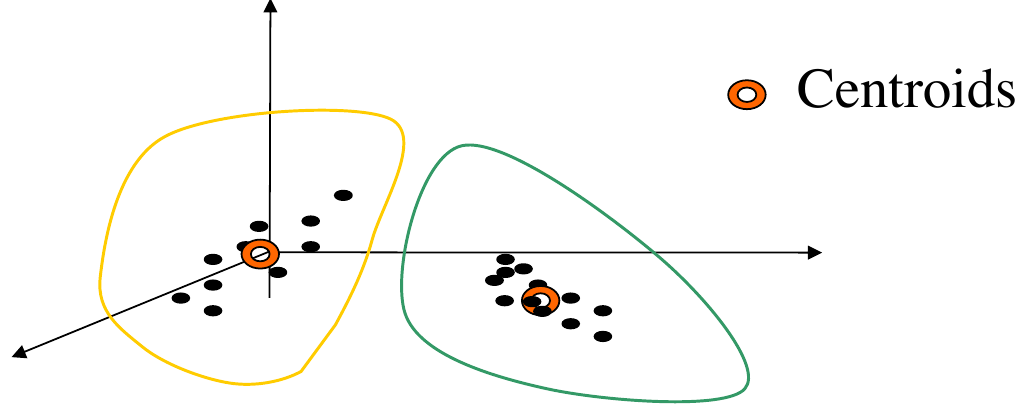
\includegraphics[width=0.54\linewidth,height=0.42\textheight,keepaspectratio]{images/03-l23_clustering.png}
\caption{Clustering: partition of the data into groups represented by
centroids.}
\end{figure}

Clustering has been tackled in a great many contexts and disciplines,
with thousands of different algorithms: this reflects its usefulness
as a step of exploratory data analysis. Here we adopt the perspective
of \textbf{vector quantization} for \textbf{partitional clustering}.

\begin{boxwarning}{The metric dominates}

As for K-NN, it is the \textbf{assumed distance} that says which
examples are similar, and the algorithm decides the groupings based on
that metric. The Euclidean distance is popular but it is \textbf{just
one choice}, and the choice can have deep implications (for example
outliers can be weighted less by using \(1 -\) a Gaussian centred on
the prototype).

\end{boxwarning}

\section{Vector quantization}\label{quantizzazione-vettoriale}

\begin{boxdefinition}{Vector Quantization (VQ)}

Vector quantization techniques encode a data manifold
\(V \subseteq \mathbb{R}^n\) using only a finite set
\(\mathbf{w} = (\mathbf{w}_1, \dots, \mathbf{w}_K)\) of reference
vectors (\emph{codebook}) \(\mathbf{w}_i \in \mathbb{R}^n\). A vector
\(\mathbf{x} \in V\) is described by the \textbf{winning} (\emph{best
matching}) reference vector \(\mathbf{w}_{i^*(\mathbf{x})}\), the one
with minimum distortion \(d(\mathbf{x}, \mathbf{w}_{i^*(\mathbf{x})})\).

\end{boxdefinition}

This divides the manifold into sub-regions, the \textbf{Voronoi
polyhedra}: \[
V_i = \{\mathbf{x} \in V \;:\; \|\mathbf{x} - \mathbf{w}_i\| \le \|\mathbf{x} - \mathbf{w}_j\| \;\forall j\},
\] and each \(\mathbf{x}\) is described by the corresponding reference
vector.

\begin{figure}[htbp]
\centering
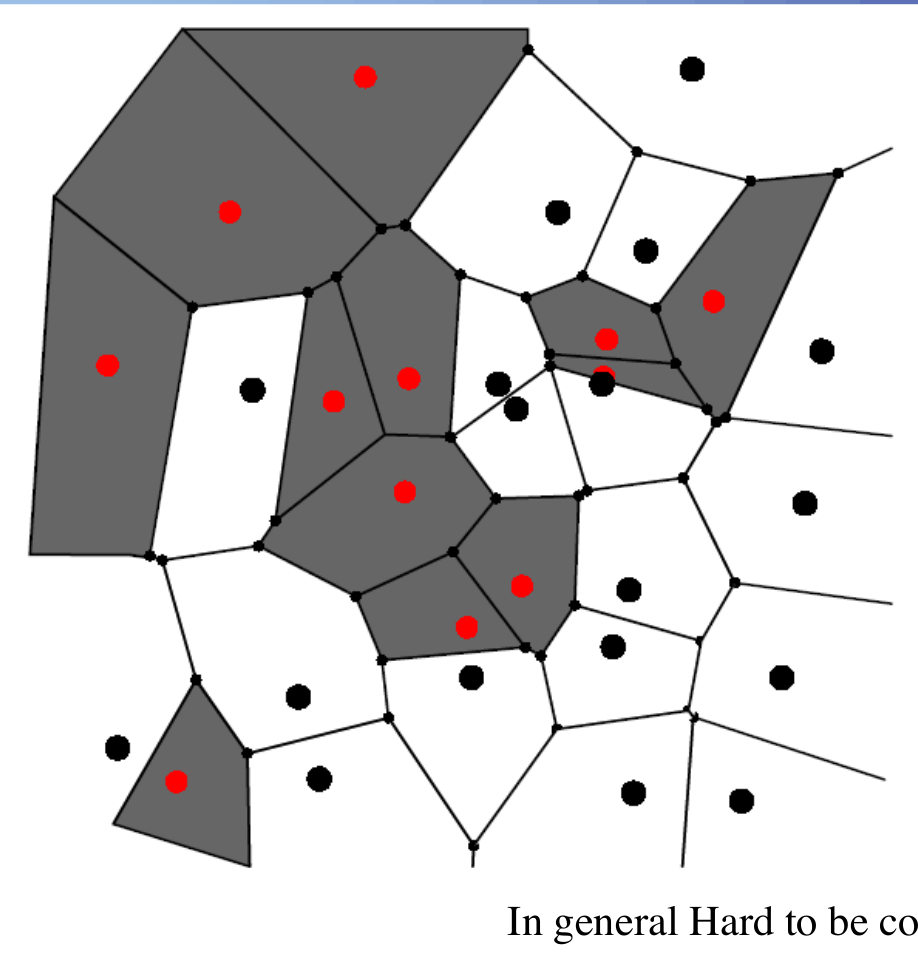
\includegraphics[width=0.43\linewidth,height=0.42\textheight,keepaspectratio]{images/19-som_voronoi.png}
\caption{Voronoi diagram: each cell contains the points closer to its
centre than to any other.}
\end{figure}

Our problem is the opposite of that of K-NN: \textbf{given the dataset,
find the centres} that minimise the loss. In general it is hard:
finding the optimal codebook is \textbf{NP-complete}.

\begin{boxexample}{Quantization in 1D}

In digital signal processing, \textbf{quantization} approximates a
continuous range of values (or a very large set of discrete values)
with a relatively small set of discrete symbols, incurring a
quantization error (distortion). This is what happens to music in
digital devices.

\begin{center}
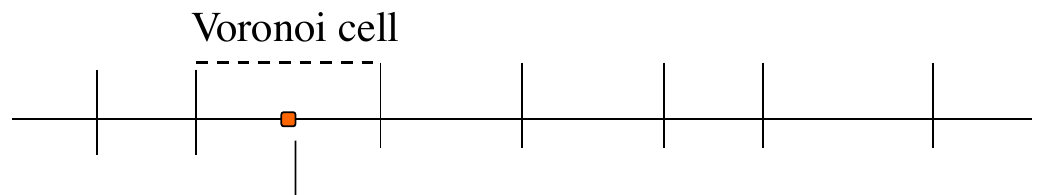
\includegraphics[width=0.54\linewidth,height=0.42\textheight,keepaspectratio]{images/19-som_quantizzazione-1d.png}
\end{center}

\end{boxexample}

\textbf{VQ and clustering.} Clustering has the more general goal of
finding \textbf{interesting or useful} groupings, where
``interesting'' is often defined implicitly by the procedure itself and
not necessarily by the minimum quantization error. However, VQ provides
a useful framework, and its algorithms are often used for clustering.

\subsection{The quantization error}\label{lerrore-di-quantizzazione}

The goal is to optimally partition an unknown distribution in the input
space into regions approximated by prototypes: a set of quantizers
\(\mathbf{x} \mapsto c(\mathbf{x}) = \mathbf{w}_{i^*(\mathbf{x})}\),
from a continuous space to a discrete one. The \textbf{squared
distortion}
\(d(\mathbf{x}, c(\mathbf{x})) = \|\mathbf{x} - c(\mathbf{x})\|^2\) is
considered; its mean value over the input distribution is the expected
distortion (or reconstruction, or quantization error). \textbf{This is
our loss}: \[
E = \int f\big(d(\mathbf{x}, \mathbf{w}_{i^*(\mathbf{x})})\big)\,p(\mathbf{x})\,d\mathbf{x} = \int \|\mathbf{x} - \mathbf{w}_{i^*(\mathbf{x})}\|^2\,p(\mathbf{x})\,d\mathbf{x},
\] where \(p(\mathbf{x})\) is the input distribution. In the discrete
version, over \(l\) data and \(K\) prototypes: \[
E = \sum_{i=1}^{l}\sum_{j=1}^{K}\|\mathbf{x}_i - \mathbf{w}_j\|^2\,\delta_{winner}(i, j), \qquad \delta_{winner}(i,j) = \begin{cases} 1 & \text{if } j \text{ is the winner for } \mathbf{x}_i \\ 0 & \text{otherwise} \end{cases}
\] (\(\delta_{winner}\) is the characteristic function of the receptive
field of \(\mathbf{w}_j\)).

Minimising \(E\) with respect to \(\mathbf{w}\) is the VQ problem.
Beware: the integrand is \textbf{not continuously differentiable},
because the winner \(\mathbf{w}_{i^*(\mathbf{x})}\) changes discretely
as \(\mathbf{x}\) varies; the derivatives are however computed
\textbf{locally}, fixing \(\mathbf{x}\) in a Voronoi cell.

\section{K-means}\label{k-means}

\subsection{On-line version}\label{versione-on-line}

Differentiating \(E\) with respect to the \(\mathbf{w}_j\) we obtain the
VQ learning rule, i.e.\ the well-known \textbf{K-means} algorithm of
Lloyd and MacQueen (on-line version): for each \(\mathbf{x}_i\), \[
\Delta\mathbf{w}_{i^*} = \eta\,\delta_{winner}(i, i^*)\,(\mathbf{x}_i - \mathbf{w}_{i^*}).
\] (The derivative of \(\|\mathbf{x}_i - \mathbf{w}_j\|^2\) with
respect to \(\mathbf{w}_j\) is \(-2(\mathbf{x}_i - \mathbf{w}_j)\);
moving in the direction opposite to the gradient brings \(\mathbf{w}_j\)
closer to \(\mathbf{x}_i\).)

\begin{itemize}
\tightlist
\item
  \textbf{Only the winning prototype} is modified, moving it towards
  \(\mathbf{x}\).
\item
  It is a stochastic gradient descent → \textbf{local minima}; the
  method depends on the \textbf{initialisation}.
\item
  The \textbf{number of clusters} must be given in advance.
\end{itemize}

\subsection{Batch version}\label{versione-batch}

\begin{boxabstract}{Batch K-means algorithm (Linde-Buzo-Gray, or generalised Lloyd)}

\begin{enumerate}
\def\labelenumi{\arabic{enumi}.}
\tightlist
\item
  Choose \(K\) centres: \(K\) randomly drawn patterns, or \(K\) random
  points in the hypervolume containing the patterns.
\item
  Assign each pattern to the closest centre (the \textbf{winner}): \[
  i^*(\mathbf{x}) = \arg\min_i \|\mathbf{x} - \mathbf{w}_i\|^2, \qquad \|\mathbf{x} - \mathbf{w}_i\|^2 = \sum_{j=1}^{n}(x_j - w_{ij})^2.
  \]
\item
  Recompute the centres as the \textbf{mean} (geometric centroid) of
  the cluster members: \[
  \mathbf{w}_i = \frac{1}{|\text{cluster}_i|}\sum_{\mathbf{x}_j \in \text{cluster}_i}\mathbf{x}_j.
  \]
\item
  If the convergence criterion is not satisfied (no or minimal
  reassignment of patterns, minimal decrease of the squared error), go
  back to step 2.
\end{enumerate}

\end{boxabstract}

(Exercise: from the on-line to the batch version. By summing --- or
averaging --- the on-line delta with \(\eta = 1\) over the patterns of a
cluster, one obtains
\(\mathbf{w}_{new} = \mathbf{w}_{old} + \frac{1}{|C|}\sum_{\mathbf{x} \in C}(\mathbf{x} - \mathbf{w}_{old}) = \frac{1}{|C|}\sum_{\mathbf{x} \in C}\mathbf{x}\):
exactly the mean.)

\begin{figure}[htbp]
\centering
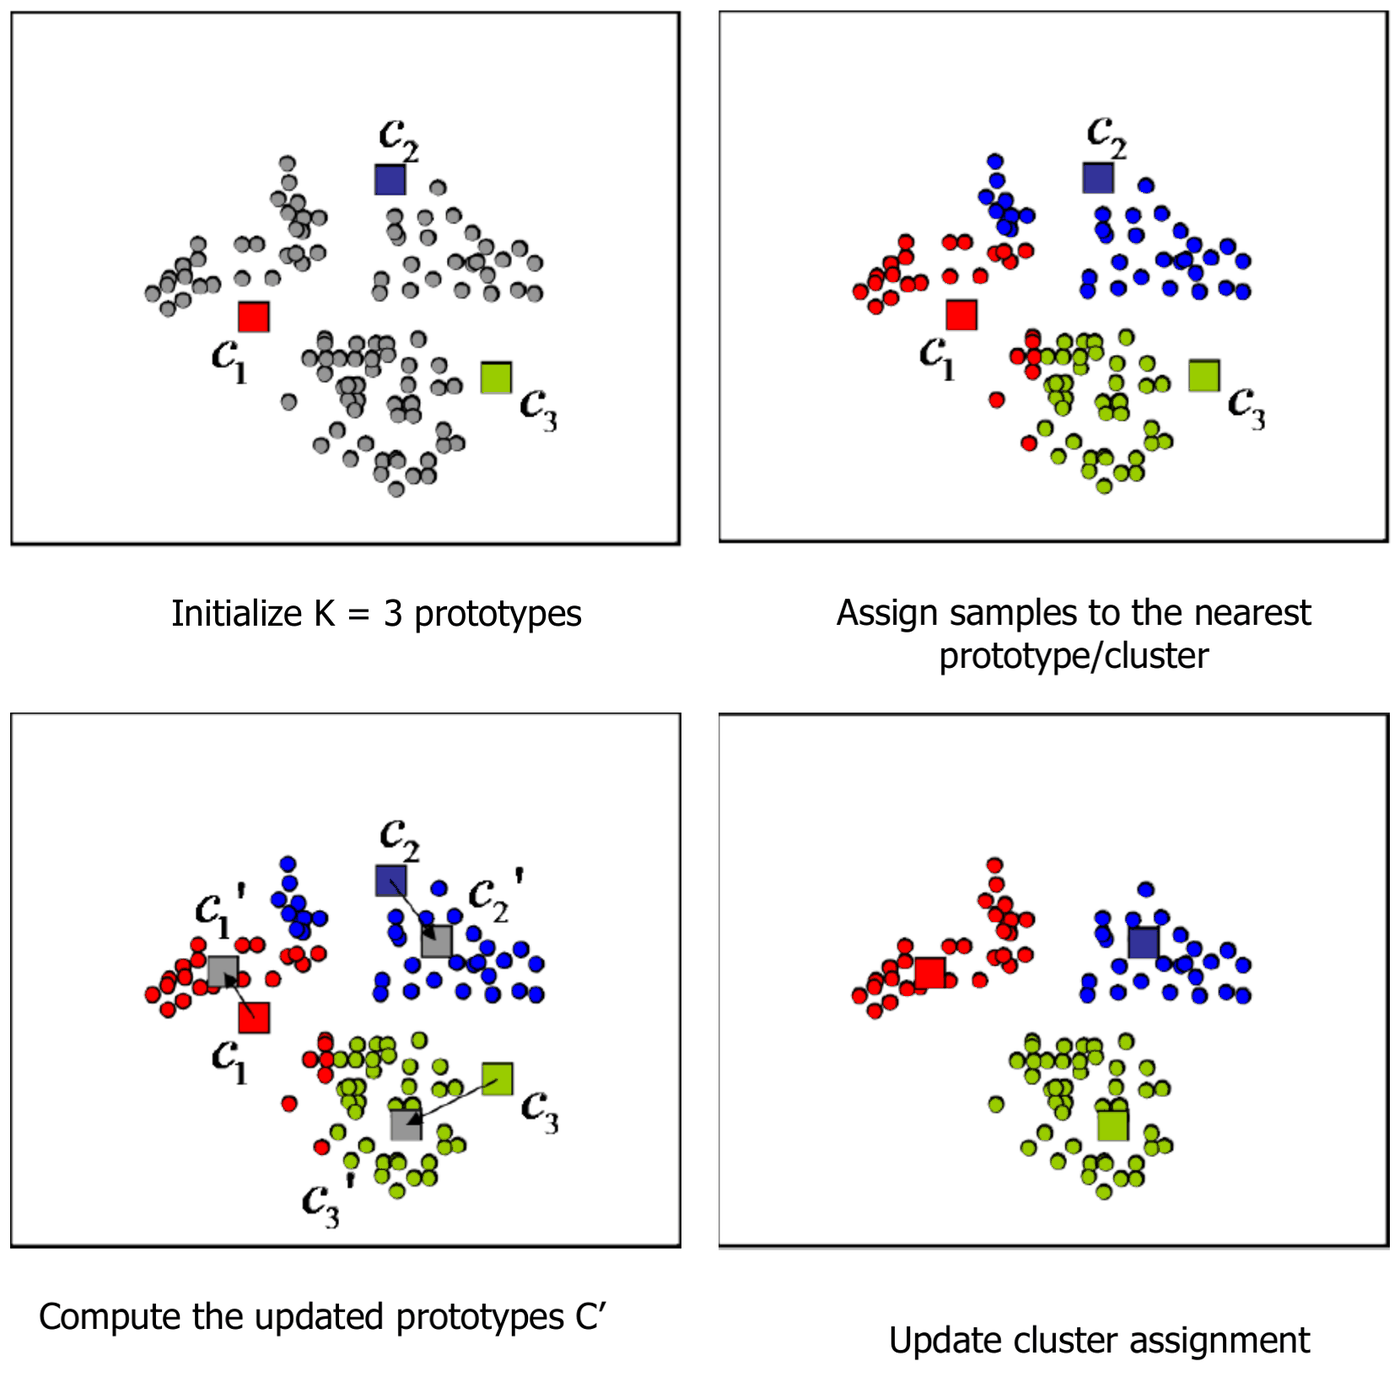
\includegraphics[width=0.80\linewidth,height=0.42\textheight,keepaspectratio]{images/19-som_kmeans.png}
\caption{K-means example with \(K = 3\): initialisation, assignment,
prototype update, new assignment.}
\end{figure}

\subsection{Strengths and weaknesses}\label{pregi-e-difetti}

\begin{itemize}
\tightlist
\item
  It is the simplest and most used algorithm with a squared error
  criterion; it is popular because it is easy to implement and
  generally efficient.
\item
  The number \(K\) of clusters must be provided.
\item
  The local minima of \(E\) make the method dependent on the
  initialisation, with only sub-optimal choices of the prototypes.
\item
  It works very well for \textbf{compact, hyperspherical} clusters;
  with clusters of other shapes (for example two intertwined
  ``spirals'') it fails.
\item
  \textbf{No visualisation property}: it does not allow projecting the
  data into a lower-dimensional space, and the indexing of the
  \(\mathbf{w}\) is arbitrary, so the mapping is not ordered.
\end{itemize}

\subsection{Soft-max}\label{soft-max}

To avoid local minima a \textbf{soft-max} adaptation rule is
introduced: not only the winner is modified, but \textbf{all} the
centres, according to their \textbf{proximity} to \(\mathbf{x}\), with
a step that decreases with the distance \(d(\mathbf{x}, \mathbf{w}_i)\)
(for example \emph{maximum-entropy clustering} with Gaussian
distances). An instance of this strategy in neural networks is
\textbf{Kohonen's SOM}, where however the proximity between reference
vectors is defined on an \textbf{ordered map}, i.e.\ a neural grid on
which they are arranged.

\section{Self-Organizing Map}\label{self-organizing-map}

\textbf{Self-Organizing Maps} (SOM), or \textbf{Kohonen maps} (1981),
are networks of \(N\) neurons arranged on a \textbf{regular
low-dimensional grid} (usually 2D, a \emph{lattice}).

\begin{itemize}
\tightlist
\item
  Each unit is identified by its \textbf{coordinates} on the map.
\item
  Each unit receives \textbf{the same input} \(\mathbf{x}\).
\item
  Each unit has a \textbf{weight} \(\mathbf{w}\), with
  \(\dim(\mathbf{w}) = \dim(\mathbf{x}) = n\).
\end{itemize}

\subsection{Goal}\label{obiettivo}

The SOM learns a map from the input space to a lattice of neural units
that \textbf{preserves the topology}:

\begin{itemize}
\tightlist
\item
  nearby units on the map respond to similar input patterns;
\item
  nearby points in the input space are mapped onto the same unit or
  onto nearby units;
\item
  the (2D) output map has \textbf{visualisation} properties.
\end{itemize}

\begin{figure}[htbp]
\centering
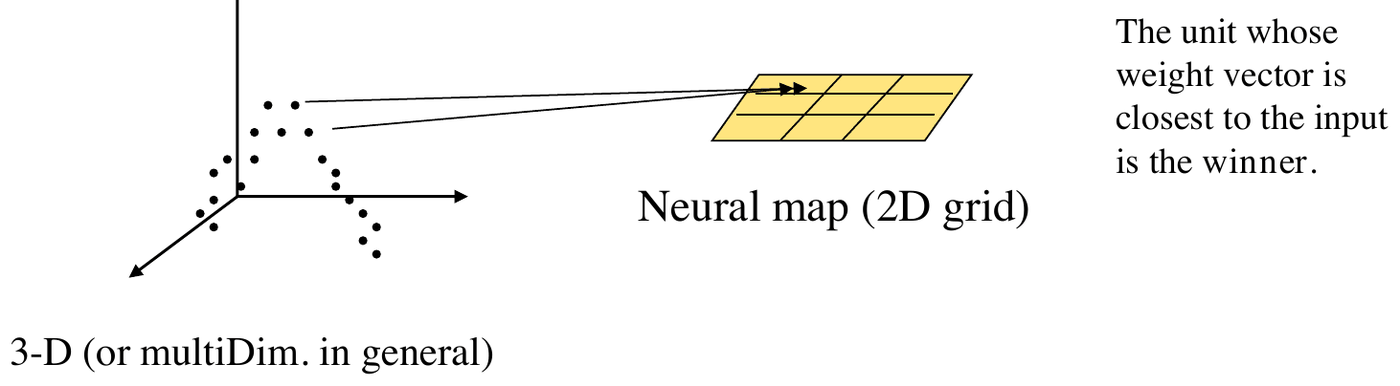
\includegraphics[width=0.74\linewidth,height=0.42\textheight,keepaspectratio]{images/19-som_mappa.png}
\caption{A SOM maps the input space (here 3D) onto a 2D neural grid.}
\end{figure}

Uses of the SOM:

\begin{itemize}
\tightlist
\item
  \textbf{clustering}: clusters are identified on the map (structures
  in the data are found quickly);
\item
  \textbf{pattern recognition and VQ}: the input is transformed into
  the weight vector of the closest neuron (the codebook vector);
\item
  \textbf{compression}: the input is transformed into the index (code)
  of the winning unit;
\item
  \textbf{projection and exploration}: the distribution of
  multidimensional data is visualised in a lower-dimensional space (the
  2D map).
\end{itemize}

\subsection{Competitive learning and biological
inspiration}\label{apprendimento-competitivo-e-ispirazione-biologica}

\textbf{Competitive learning} is an adaptive process in which neurons
gradually become sensitive (specialised) to different categories or
sets of inputs: neurons \textbf{compete} for a data point, and the
winner learns the most.

Nature exploits this mechanism: in the \textbf{somatosensory} (and
motor) \textbf{cortex} there is a \textbf{topologically ordered} map of
the body, the \textbf{homunculus}. Adjacent neurons represent nearby
activation sources in the body, and the most sensitive parts occupy
larger areas of the cortex. In a topology-preserving map, physically
close units respond to classes of inputs that are in turn close.

\begin{figure}[htbp]
\centering
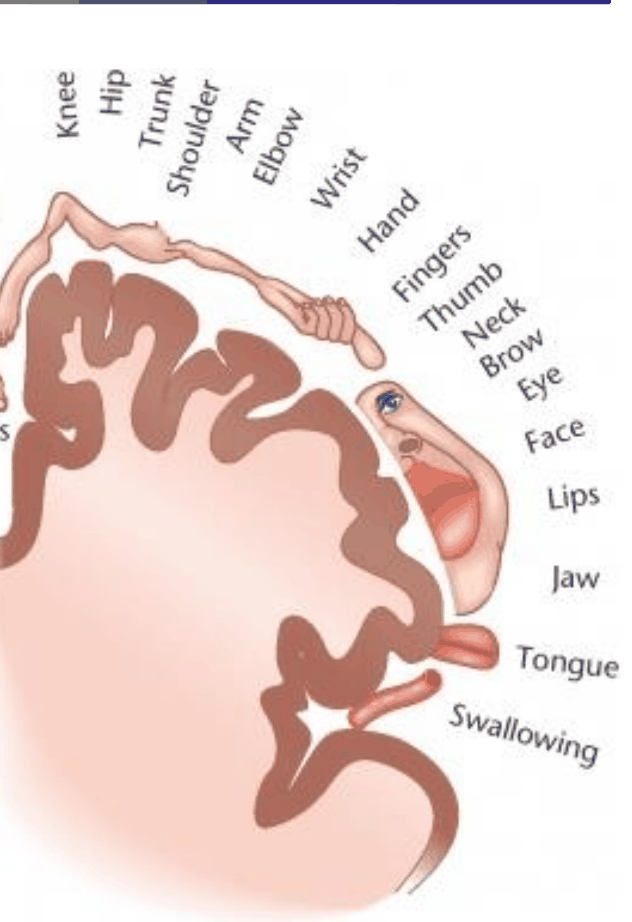
\includegraphics[width=0.31\linewidth,height=0.42\textheight,keepaspectratio]{images/19-som_homunculus.png}
\caption{The homunculus: a topologically ordered map of the body in the
cortex.}
\end{figure}

\subsection{The algorithm}\label{lalgoritmo}

\begin{boxabstract}{SOM algorithm}

\begin{itemize}
\tightlist
\item
  Randomly initialise the weights of the map.
\item
  Draw an input \(\mathbf{x}\).
\item
  \textbf{Competitive phase}: the winner is the unit with
  \(\mathbf{w}\) most similar to \(\mathbf{x}\).
\item
  \textbf{Cooperative phase}: update the weights of the units that have
  topological relations \textbf{on the map} with the winner (a form of
  soft-max).
\item
  Continue until convergence (no change).
\end{itemize}

\textbf{Key factor}: the neighbours \textbf{on the map} (whereas
standard soft-max uses proximity in the data space).

\end{boxabstract}

\subsubsection{Competitive phase}\label{fase-competitiva}

The input \(\mathbf{x}\) is compared with the weights of all units with
the Euclidean distance. The standard SOM adopts a
\textbf{winner-take-all} strategy (like K-means): \[
i^*(\mathbf{x}) = \arg\min_i \|\mathbf{x} - \mathbf{w}_i\|,
\] where \(i\) is an index on the map (for example the 2D coordinates).

\subsubsection{Cooperative phase}\label{fase-cooperativa}

The weights of the winner \textbf{and of the units in its
neighbourhood} are moved towards the input (Hebbian learning). At
iteration \(t\): \[
\mathbf{w}_i(t+1) = \mathbf{w}_i(t) + \eta(t)\,h_{i,i^*(\mathbf{x})}(t)\,\big[\mathbf{x} - \mathbf{w}_i(t)\big],
\] where \(h\) is the \textbf{neighbourhood function}
(\emph{neighborhood kernel}), which decreases monotonically as the
distance \textbf{on the map} between unit \(i\) and the winner
increases. For example a Gaussian: \[
h_{i,i^*}(t) = \exp\left(-\frac{\|\mathbf{r}_i - \mathbf{r}_{i^*}\|^2}{2\sigma^2(t)}\right),
\] with \(\mathbf{r}_i\) the coordinates of unit \(i\) on the grid and
\(\sigma(t)\) the width.

The \textbf{learning rate} \(\eta\) and the \textbf{neighbourhood
radius} \(\sigma\) decrease with the iterations: the neighbourhood is
\textbf{wide at the beginning} (global ordering of the map) and then
shrinks slowly during learning (convergence, local refinement). In
practice the shape of the neighbourhood is chosen among standard
geometric shapes on the grid (rectangular, hexagonal\ldots) that
include a finite set of units.

\subsection{The emergence of topological
order}\label{lemergere-dellordine-topologico}

The cooperative phase rule is \textbf{fundamental} for the formation of
topographically ordered maps. The weights are not modified
independently, but \textbf{in topologically related subsets}: at each
step the neighbourhood of the winner on the grid is selected, and all
units in the subset receive similar updates. In this way topological
information is transmitted to the map: the winner and its neighbours on
the grid receive similar updates and, after learning, respond to
similar inputs. Even though it seems natural, a formal proof of the
ordering is difficult.

\begin{boxtip}{K-means versus SOM}

\begin{itemize}
\tightlist
\item
  \textbf{K-means}: updates only the winner; the prototypes have no
  order; there is no visualisation.
\item
  \textbf{SOM}: updates the winner \textbf{and its neighbours on the
  grid}, with a neighbourhood that shrinks over time; the prototypes are
  arranged on an ordered map that \textbf{preserves topology}, allowing
  visualisation; the initially wide neighbourhood also helps avoid local
  minima. (With a zero-radius neighbourhood, the SOM reduces to on-line
  K-means.)
\end{itemize}

\end{boxtip}

\begin{figure}[htbp]
\centering
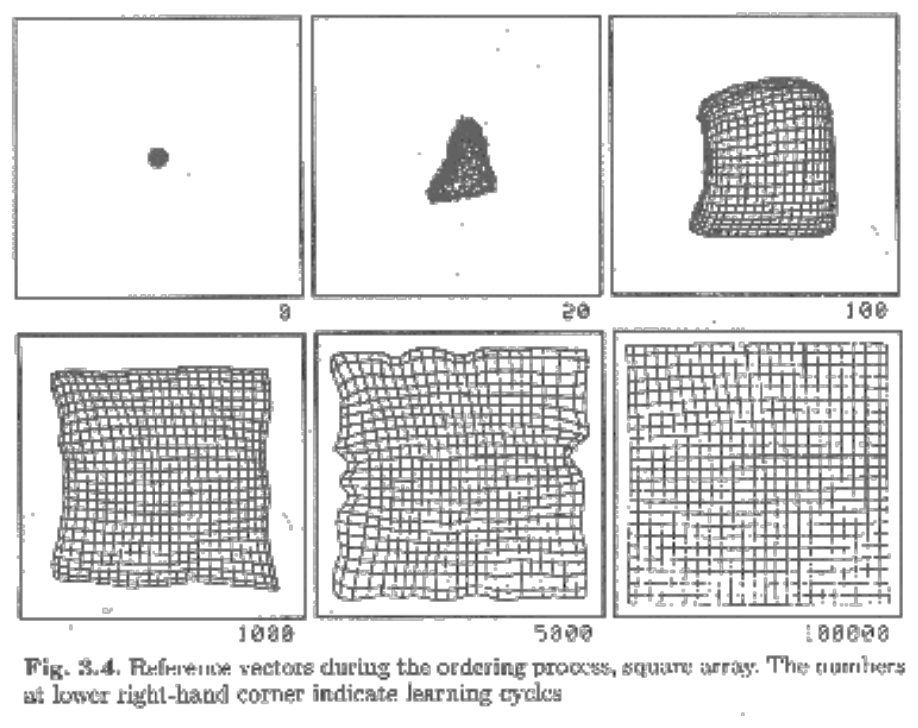
\includegraphics[width=0.69\linewidth,height=0.42\textheight,keepaspectratio]{images/19-som_training-uniforme.png}
\caption{Training a SOM on uniform 2D data: the reference vectors
(connected according to the grid) progressively unfold over the
distribution.}
\end{figure}

During training the units ``come to represent'' the clusters of the
data.

\subsection{Visualisation}\label{visualizzazione}

The map can be used to visualise various characteristics of the SOM and
of the data:

\begin{itemize}
\tightlist
\item
  the \textbf{density} of the reference vectors (colour proportional to
  the number of ``hits'');
\item
  the \textbf{distances} between the prototypes of neighbouring units
  (\textbf{U-matrix}): dark colours indicate large distances between
  adjacent units, light colours small distances;
\item
  Sammon maps (with lines)\ldots{}
\end{itemize}

This makes the SOM easily \textbf{interpretable}.

\begin{boxexample}{Welfare and poverty in the world (Kaski and Kohonen, 1995)}

39 welfare indicators for 77 countries (World Development Report 1992).
On the 13×9 map, the grey level between two units indicates the (scaled
and smoothed) distance between their reference vectors: light areas are
clusters of similar countries, dark areas the borders between clusters.
No a priori assumption on the shape of the clusters is needed.

\begin{center}
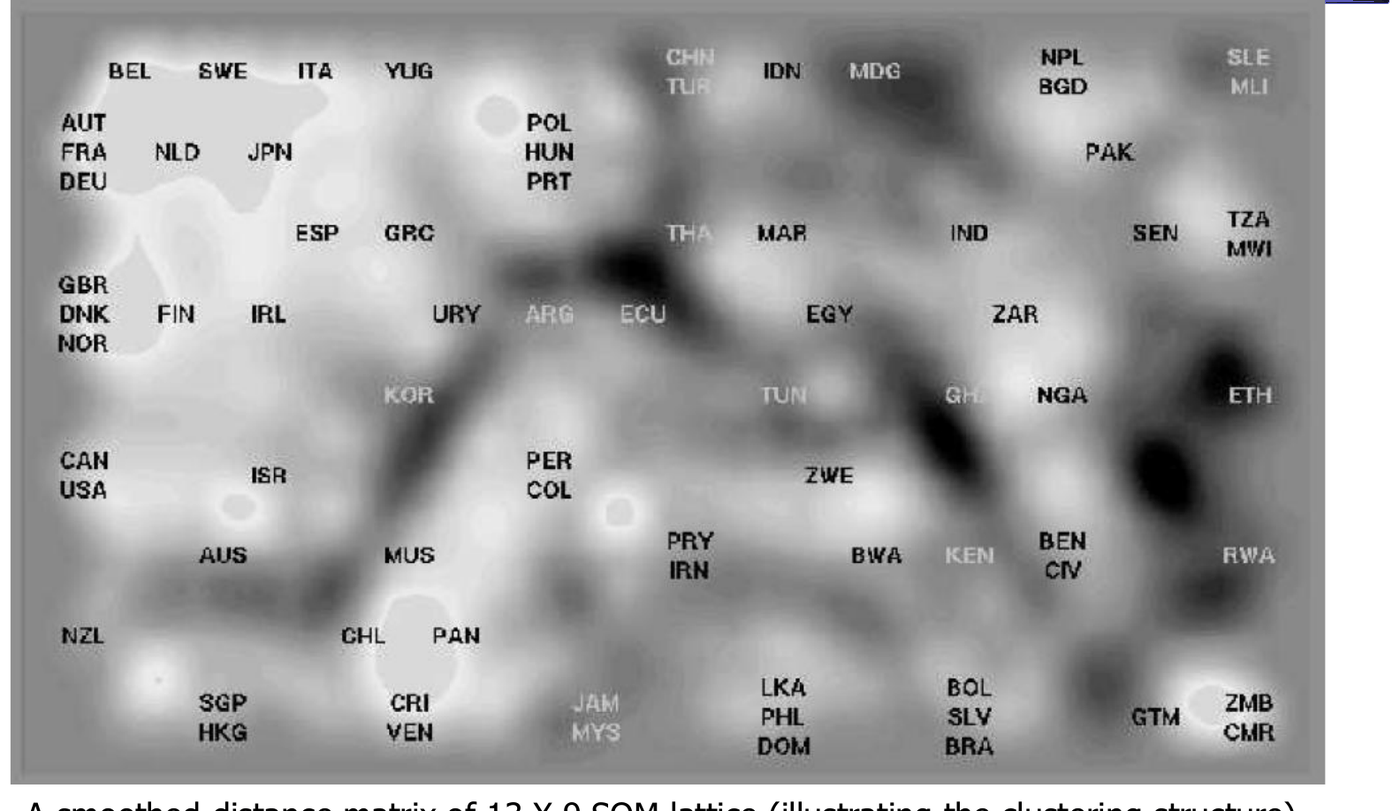
\includegraphics[width=0.80\linewidth,height=0.42\textheight,keepaspectratio]{images/19-som_umatrix.png}
\end{center}

\begin{center}
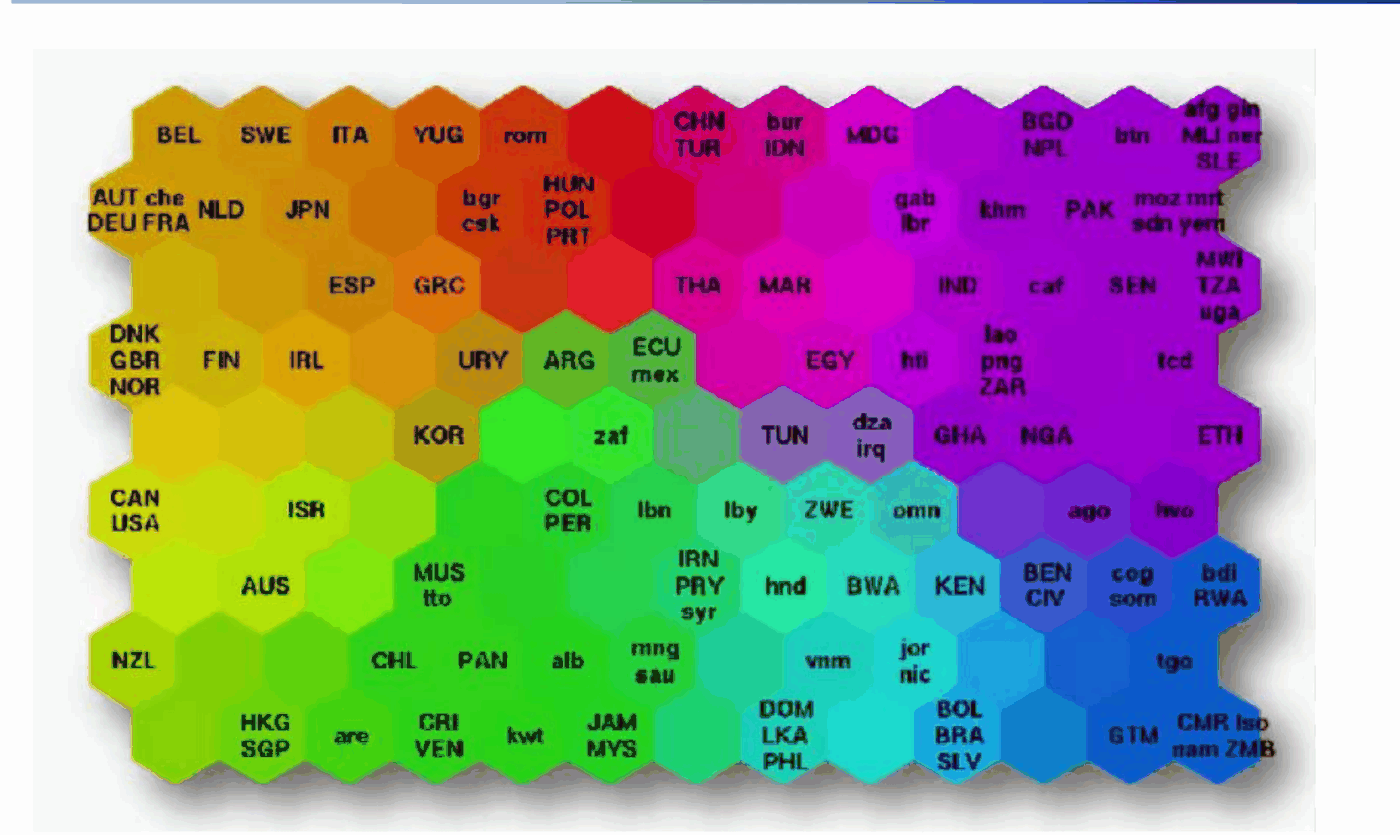
\includegraphics[width=0.80\linewidth,height=0.42\textheight,keepaspectratio]{images/19-som_mappa-colori.png}
\end{center}

\end{boxexample}

\section{Evaluating a clustering
(outline)}\label{valutare-un-clustering-cenni}

How is the result of a clustering evaluated? What distinguishes a good
result from a poor one?

\begin{itemize}
\tightlist
\item
  Evaluation is often \textbf{subjective}: there are few ``gold
  standards'', except in well-defined sub-domains.
\item
  \textbf{Objective} measures, such as the quantization error (which
  however depends on the number of centroids).
\item
  One does \textbf{not} trivially use the label of an underlying
  classification task (\emph{purity}, with entropy, mutual
  information\ldots): if labels are available, one might as well use a
  classifier.
\item
  Quality of the model/clustering versus quality of the results
  (domain-dependent).
\end{itemize}

Other topics in unsupervised learning: hierarchical clustering
(dendrograms), principal component analysis (and principal curves and
surfaces), association rules, ICA, Multidimensional Scaling, t-SNE,
Generative Topographic Mapping, ART networks.

\begin{boxquestion}{Possible exam questions}

\begin{itemize}
\tightlist
\item
  Define clustering and vector quantization. What is the quantization
  error?
\item
  Derive the on-line K-means rule and move to the batch version.
\item
  Strengths and weaknesses of K-means.
\item
  Describe the SOM: architecture, competitive phase, cooperative phase,
  neighbourhood function.
\item
  Why does the SOM preserve topology? Differences between K-means and
  SOM.
\item
  How is a SOM visualised (U-matrix)?
\end{itemize}

\end{boxquestion}
